\documentclass[10pt]{article}
\usepackage{geometry}
\geometry{letterpaper, top=2cm, right=4cm, left = 4cm} 
\usepackage{amssymb}
\usepackage{amsmath}
\usepackage{hyperref}
\usepackage{xspace}
\usepackage{xcolor}
\usepackage{graphicx}
\usepackage{float} % Place figures exactly "here" (option "H")
\usepackage[modulo]{lineno}
\hypersetup{
colorlinks=true,
linkcolor = blue,
citecolor = blue} 


\bibliographystyle{apalike}

% ==== My Macro =====


\newcommand{\warning}[1]{\textbf{\textcolor{orange}{((#1))}}}
\newcommand{\comment}[1]{\textsl{\textcolor{cyan}{((#1))}}}
\newcommand{\sq}[1]{\texttt{\textcolor{brown}{#1}}}
\newcommand{\pr}[1]{\mathrm{Pr}(#1)}
\newcommand{\betadist}[1]{\mathrm{Beta}\left(#1\right)}
\newcommand{\eg}{\textit{e.g.,}\xspace}
\newcommand{\ie}{\textit{i.e.,}\xspace}

\newcommand{\sps}{\mathcal{B}} % sequence probability sequence
\newcommand{\nps}{\mathcal{S}} % nucleotide probability sequence
\newcommand{\nlps}{nucleotide-level probabilistic sequence\xspace}
\newcommand{\slps}{sequence-level probabilistic sequence\xspace}


% ===================

\title{Propagating Sequence Uncertainty in Phylogeny Reconstruction}
\author{Champredon, David \and Poon, Art}
\date{\today}

\begin{document}
\maketitle
\linenumbers

\section{Introduction}

Molecular phylogenies are tree-based models that relate common ancestors of genetic sequences.
Many sophisticated statistical tools exist to reconstruct phylogenies from genetic material extracted from biological samples. 
Those statistical methods rely, to a varying degree, on ``truthful'' and accurate observations of molecular sequences, their main -- if not unique -- input data.

\textbf{Sequencing error.} 
Extracting DNA/RNA from biological samples is a complex process that involves several steps: extraction of the genetic material of interest (avoiding contamination with foreign/unwanted genetic material); reverse transcription (if RNA); DNA fragmentation of the genome into smaller segments; amplification of the fragmented sequences using PCR; sequencing the fragments (\eg with fluorescent techniques); putting back the small fragments together by aligning them (de novo) or mapping them to benchmark libraries.\comment{(all this must be checked by someone who knows well the process!)}
Errors can be introduced at each of these steps for various reasons \cite{Beerenwinkel:2011} and some errors can be quantified (\eg sequencing quality scores from chromatographs). 

\textbf{In-host diversity and polymorphisms.} 
When the phylogenic tree to infer is based on pathogen sequences infecting hosts, the potential genetic diversity of the infection adds a complexity in phylogeny reconstruction. Typical examples are epidemiological studies reconstructing transmission trees from viral genetic sequences (\eg HIV, HepC) sampled from infected patients \comment{ref phyloscanner}. 


\textbf{Current uncertainty management.} 
The different sources of uncertainty described above impact our observations of the actual genetic sequences.
There are standard approaches to deal with identifiable observation errors. 
Base calls that are ambiguous (from equivocal chromatograph curves or because of genuine polymorphisms) are assigned ambiguity codes (\eg Y for C or T, R for A or G, etc.).
Alignment methods are heuristic methods based on similarity scores that generally do not quantify the uncertainty of alignment.\comment{double check this is indeed the case for MUSCLE, MAPFT, PRANK, ClustalW}
Methods to reconstruct phylogenies usually leave out the uncertainty complexity and settle for sequences composed of the most frequent nucleotides and/or ignore ambiguity codes.

\textbf{Propagate and quantify uncertainty.}
In summary, sources of sequencing observation errors are known and, for a few of them, quantified (quality scores, ambiguity codes).
But, to our knowledge, the resulting uncertainty has never been propagated and quantified in a statistical framework for downstream analysis in  phylogenies inferences.
\comment{Check what BALIphy does, this may be the only example of uncertainty propagation}
In other words, genetic sequences are treated as \emph{certain} quantities.

Here we propose a theoretical framework to represent genetic sequence uncertainty and quantify the impact of uncertainty as it is propagated through methods of phylogeny reconstruction. 



% ==============================================================
% ==============================================================




\section{Methods}



\subsection{Probabilistic sequences}

Here, we propose two simple probabilistic frameworks to represent the uncertainty of our genetic sequences observations.
The first framework represents uncertainty at the \emph{nucleotide level}, whereas the second one is at the \emph{sequence level}.
In both frameworks, the sequence of nucleotides from a biological sample is not treated as a certain observation anymore, but as a collection of possible sequences.


\subsubsection{Nucleotide-level uncertainty}
 
We define probabilistically a nucleotide sequence in a matrix form. For a sequence of length $\ell$ we can write:

$$\nps = \bordermatrix{   & 1 & 2 & \ldots & \ell \cr
                \sq{A} & \nps_{A, 1} & \nps_{A, 2} & \ldots & \nps_{A, \ell} \cr
                \sq{C} & \nps_{C, 1} & \nps_{C, 2} & \ldots & \nps_{C, \ell} \cr
                \sq{G} & \nps_{G, 1} & \nps_{G, 2} & \ldots & \nps_{G, \ell} \cr
                \sq{T} & \nps_{T, 1} & \nps_{T, 2} & \ldots & \nps_{T, \ell} \cr 
                \sq{-} & \nps_{x, 1} & \nps_{x, 2} & \ldots & \nps_{x, \ell} \cr 
}$$
Each column represents the nucleotide position, each row one of the four nucleotide \sq{A,C,G,T} as well as an empty position ``\sq{-}'' that symbolizes a genuine deletion (not caused by missing data).
Hence, $\nps$ is a $5\times\ell$ matrix. Its elements represent the probability that a nucleotide is at given position:

\begin{equation}
\nps_{n,j} = \pr{\text{nucleotide \sq{n} is at position }j}
\end{equation}
with the special case for a deletion:

\begin{equation}
\nps_{\sq{-},j} = \pr{\text{empty position }j}
\end{equation}
Note that we have for all $1\leq j \leq \ell$:
\begin{equation}
\sum_{n\in \{ \sq{A,C,G,T,-} \} } \nps_{n, j} = 1
\end{equation}
Also, the sequence length is stochastic if $\nps_{x,i}>0$ for at least one $i$. The probability that the sequence has the maximum length $\ell$ is $\prod_{i=1}^\ell (1-\nps_{x,i})$. 
We call the matrix $\nps$ the \emph{\nlps} of a biological sample.
The nucleotide (or deletion) drawn at each position is independent from all the other one, so there are $5^\ell$ possible different sequences for a given probabilistic nucleotide sequence. 



\subsubsection{Sequence-level uncertainty}

Out of the $5^\ell$ possible sequences, the nucleotide uncertainty likely assigns a positive probability to sequences that are not biologically possible.
As an alternative representation and to reduce the space of sequences, let's assume we have enough information (either directly observed from data or simulated) to generate a set of $m$ sequences $\sps = (\sps_i)_{i\in\{1\ldots m\} }$ of all biologically possible sequences. Note that the $\sps_i$ do not have necessarily the same length. 
The observed genetic sequence, $s$, is a sample from a specified distribution $a$:
\begin{equation}
\pr{s = \sps_i} = a(i)
\end{equation}
We call the set $\sps$ the \emph{\slps}.




\subsubsection{Examples}

If we have the following \nlps:
$$
\nps = 
\bordermatrix{
& \scriptscriptstyle{1} & \scriptscriptstyle{2}& \scriptscriptstyle{3}& \scriptscriptstyle{4} & \scriptscriptstyle{5} & \scriptscriptstyle{6} \cr
\sq{A} & 0.9 & 0.05   & 0.99 & 0 & 0 & 0.6\cr
\sq{C} & 0   & 0.8 & 0 & 0 & 0.1 & 0.1\cr
\sq{G} & 0.1 & 0.15 & 0 & 0.3 & 0.9 & 0\cr
\sq{T} & 0 & 0 & 0.01 & 0.7 & 0 & 0.3\cr
\sq{-} & 0 & 0 & 0 & 0 & 0 & 0\cr
}
$$
then there are $2\times 3 \times 2^3 \times 3 = 144$ possible sequences. The most likely is the one having the highest nucleotides probabilities: \sq{ACATGA} with probability 0.2694  ($0.9\times 0.8\times 0.99 \times 0.7 \times 0.9 \times 0.6$).

If there is a positive probability of deletion for at least one position, then the sequence has a variable length. 
Let's take the same example as above, but adding one possible empty position:

$$
\nps = 
\bordermatrix{
&\scriptscriptstyle{1} & \scriptscriptstyle{2}& \scriptscriptstyle{3}& \scriptscriptstyle{4} & \scriptscriptstyle{5} & \scriptscriptstyle{6} \cr
\sq{A} & 0.9 & 0.05   & 0.99 & 0 & 0 & 0.6\cr
\sq{C} & 0   & 0.8 & 0 & 0 & 0.1 & 0.1\cr
\sq{G} & 0.1 & 0.15 & 0 & 0.2 & 0.9 & 0\cr
\sq{T} & 0 & 0 & 0.01 & 0.7 & 0 & 0.3\cr
\sq{-} & 0 & 0 & 0 & 0.1 & 0 & 0\cr
}
%\begin{pmatrix}
%0.9 & 0.05   & 0.99 & 0 & 0 & 0.6\\
%0   & 0.8 & 0 & 0 & 0.1 & 0.1\\
%0.1 & 0.15 & 0 & 0.2 & 0.9 & 0\\
%0 & 0 & 0.01 & 0.7 & 0 & 0.3\\
%0 & 0 & 0 & 0.1 & 0 & 0\\
%\end{pmatrix}
$$

\noindent Like above, there is still a 0.2694 probability that the sequence is \sq{ACATGA}, but now there is a chance that position 4 is deleted. For example, with probability 0.038 the sequence is \sq{ACA-GA}.

Let's take the following example for a \slps $\sps$:
\begin{table}[H]
%\caption{default}
\begin{center}
\begin{tabular}{lc}
\hline
sequence & $a$ \\
\hline
\sq{ACATGA} & 0.60 \\
\sq{ACATCA} & 0.12 \\
\sq{AGATCA} & 0.15 \\
\sq{ACAGA}  & 0.05 \\
\sq{GCATGA} & 0.08 \\
\hline
\end{tabular}
\end{center}
\label{default}
\end{table}%
Sampling from $\sps$, we will have for example \sq{ACATCA} $12\%$ of the time. 


\subsection{Probabilistic sequences from data}

Here, we suggest possible methods to populate values in probabilistic sequences from data. 

\subsubsection{Quality scores}
Fragment sequencing error is an error that is quantified with quality (or ``Phred'') score attributed to each base call from sequencing instrument. 
The quality score $Q$ is directly related to the error probability: $\epsilon = 10^{-Q/10}$ \cite{xxx} (for the widespread Illumina instruments, the sequencing error probability ranges between $10^{-3.5}$ and  $10^{-1.5}$ \cite{xxx}).  
So each base call is right with probability $1-\epsilon$. Assuming the other bases and deletion \sq{-} are all equally likely with probability $\epsilon/4$. Alternatively, if we know only mutations (not deletions) affect the sequence, the last row can be filled with zeros and the other base-calls equal to $\epsilon/3$.

For example, let's assume the output sequence after fragment sequencing and alignment is \sq{ACATG} and its associated quality scores are respectively $Q=60,30,50,10,40$. The probabilistic sequence can be defined as:

$$
S = 
\begin{pmatrix}
1-10^{-6} & 10^{-3}/4  & 1-10^{-5} & 10^{-1}/4 & 10^{-4}/4  \\
10^{-6}/4 & 1-10^{-3}  & 10^{-5}/4 & 10^{-1}/4 & 10^{-4}/4  \\
10^{-6}/4 & 10^{-3}/4  & 10^{-5}/4 & 10^{-1}/4 & 1-10^{-4} \\
10^{-6}/4 & 10^{-3}/4  & 10^{-5}/4 & 1-10^{-1} & 10^{-4}/4\\
10^{-6}/4 & 10^{-3}/4  & 10^{-5}/4 & 10^{-1}/4 & 10^{-4}/4 \\
\end{pmatrix}
$$
Usually, this output from the sequencing instrument would be considered as certain (and quality scores discarded). In the probabilistic sequence framework, the probability to have \sq{ACATG} is 0.899 ${\displaystyle(=(1-10^{-6})\times (1-10^{-3})\times (1-10^{-5})\times (1-10^{-1})\times (1-10^{-4}))}$.

\subsubsection{Polymorphisms data}
Both \nlps and \slps can be generated using error-only non-polymorphic data as well as data from studies investigating polymorphisms.
The design of the latter studies may vary but a standard data format they generate can be summarized as follow: the genetic material from several specimens of organisms of interests (e.g., a pathogen infecting a host) is sequenced and all polymorphisms encountered are recorded (after alignment). 
After alignment, the data can be displayed in a matrix where the columns represent the nucleotide position, the rows represent the nucleotide and deletion, and the matrix elements the number of times the nucleotide was found at that position.
If this matrix is normalized column-wise, we obtain the \nlps introduced earlier. 
An example of such a study, that we'll use to run our simulations, can be found in \cite{Zanini:2015}. \comment{other similar examples?}

\comment{Example of studies with full length sequences and their respective frequencies?}


\subsection{Propagating sequence uncertainty in phylogeny reconstruction}

Here, we describe our study design to propagate and measure sequence uncertainty in phylogeny reconstruction. 


\subsubsection{Generating simulated probabilistic sequences} 

If we want to simulate realistic probabilistic sequence, we have to reproduce a similar uncertainty as the one we would have from either sequencing error or polymorphism. 

We illustrate our methodology in the context of in-host HIV infections. 
The data from Zanini \cite{Zanini:2015} is a good source to assess primarily the diversity of polymorphism for HIV, and to a certain extent too, the sequencing error (because it is always here). 
Briefly, this data set gives, for several patients at several time points during their (untreated) infection, the number of times nucleotides were sample at a given position, across the whole HIV genome. 
The number of nucleotide occurrences at each position can easily be transformed into the probabilities for the probabilistic sequence. The entropy can then be calculated at each position, and also for the entire genome (by simply summing up the entropies for all positions). 

Entropy is a measure of uncertainty. So we can consider the distribution of entropies (for each position on the genome) as a representation of the overall genome sequencing uncertainty, that should be approximately matched by simulations deemed realistic. 
The data from Zanini shows that $\nps_{n,j}$, the distribution of base-call probabilities for most positions is highly concentrated just under 1 (which means a high base-call probability for most positions). 
Hence, we choose a Beta distribution to simulate base-call probabilities, and fit the shape parameters $\alpha$ and $\beta$ on the observed entropy distribution:
\begin{equation}
\label{eq:beta_sampling}
S_{n,j} \sim \betadist{\alpha, \beta}
\end{equation}
\begin{equation}
\alpha, \beta \text{ such that } E(\alpha,\beta) = E_{obs}
\end{equation}
where $E$ is the distribution of position-wise entropy.
A fit on Zanini's data \cite{Zanini:2015} gives approximately $\hat{\alpha} = 29.7$ and $\hat{\beta} = 0.06$. \comment{make an appendix to show the details of this fit.}

We calculate the entropy value as 
\begin{equation}
\label{eq:entropyDefinition}
E(\alpha, \beta) = -\sum_{i=1}^{\ell} p_i \log_2(p_i)
\end{equation}
where $p_i$ is the ($\alpha$- and $\beta$-dependent) base-call probability drawn for the nucleotide at position $i$ and $\ell$ is the length of the sequence.




\subsubsection{Assessing the impact of sequencing uncertainty}


Below is our simulation design to study the impact of uncertainty on phylogeny reconstruction.
An illustration of this pipeline is given by \autoref{fig:pipeline}.

\begin{enumerate}
\setcounter{enumi}{-1} 

\item Choose a root sequence of interest (\eg a HIV genome, a random sequence)

\item Generate a phylogeny from this root sequence, using \textsf{phyloSim}. The resulting tree $T^*$ has $n$ tips that represent the sequenced samples $seq_1, seq_2,\ldots, seq_n$. The tree $T^*$ with its sequences $seq_i$ is the ``base'' phylogeny.

\item Add a simulated layer of uncertainty by transforming the ``base'' sequences $seq_i$ into probabilistic sequences $\nps^i$ (for $i=1,2,\ldots,n$).

\item Repeat $M$ times: 
draw a sequence $\widetilde{seq_i}$ for each $\nps^i$ (for $i=1,\ldots, n$).

\item Repeat $M$ times: reconstruct the phylogeny $T_m$ with \textsf{RAxML} from the $(\widetilde{seq_i})_{i=1\ldots n}$. 

\item \label{item:assess} Assess the uncertainty by considering the variance among the phylogenies $(T_m)_{m=1:M}$ using several distance metrics (detailed below).
\end{enumerate}

\noindent Note that the $M$ iterations amounts to a Monte-Carlo algorithm.
Studying the distance between the $(T_m)_{m=1:M}$ and $T^*$ is not our main goal (this distance essentially assesses the performance of the phylogeny reconstruction software to correctly infer the ``true'' ancestry).
Instead, we are principally interested in \emph{uncertainty propagation}, that is the variance of the pairwise distances between the $(T_m)_{m=1:M}$.

Our analysis considers five levels of uncertainty. We start with a virtually inexistent sequence uncertainty, then increased it by lowering the base call probability. This is done by sampling the probability from multiple parameter sets $(\alpha,\beta)$ of a Beta distribution (see \autoref{eq:beta_sampling}). 
We choose a single value $\alpha=29$ and use five different values for the second shape parameter $\beta = 10^{-3}, 10^{-2}, 10^{-1}, 1 \text{ and } 3$ \comment{update if necessary}.
With these values, mean of the Beta distribution for the base-call probability decreases away from 1.0. 
Finally, note that the middle value $(\alpha=29, \beta=10^{-1})$ is close to the fitted entropy values of the longitudinal HIV dataset from Zanini and colleagues \cite{Zanini:2015}.

For Step \ref{item:assess}, we explore the impact of sequence uncertainty on several types of downstream analysis on reconstructed phylogenies: pairwise distance between trees, clustering and an example of source attribution \comment{amend if needed}.


\textbf{Pairwise distances between trees.}
Define the set 
\begin{equation}
D = \{d(T_i,T_j);\,\, i=1,\ldots, M \text{ and } j<i \}
\end{equation}
with $d$ a tree distance. 
%$D$ has ${M(M-1)/2}$ data points. 
The distance $d$ should be a statistically-convenient metric that represents faithfully the differences of interpretation (\ie uncertainty) of phylogeny reconstruction. 
We use three distances:  Robinson-Foulds (RF) \cite{Robinson:1981}, kernel \cite{Poon:2013} and a label-based distance \cite{xxx}. 
% We expect the mean (and variance) of $D$ to increase as the sequencing uncertainty increases. 

We measure the uncertainty of phylogenetic inference with the coefficient of variation $c = s / m$ where $m$ is the mean of $D$ and $s$ its standard deviation.
We note $c_{RF}$, $c_K$ and $c_{L}$ the coefficients of variation calculated with the RF, kernel and label-based distances, respectively.

Although not our primary objective in this study, we also investigate the distance of the inferred tree $T_i$ to the benchmark tree $T^*$, and define 
\begin{equation}
D^* = \{d(T_i,T^*);\,\, i=1,\ldots, M \} 
\end{equation}
Similarly as for $c$, we define $c^*$ as the coefficient of variation of $D^*$ and adopt the same subscript notation to differentiate between the distances used for its calculation.



\begin{figure}[ht]
\centering
    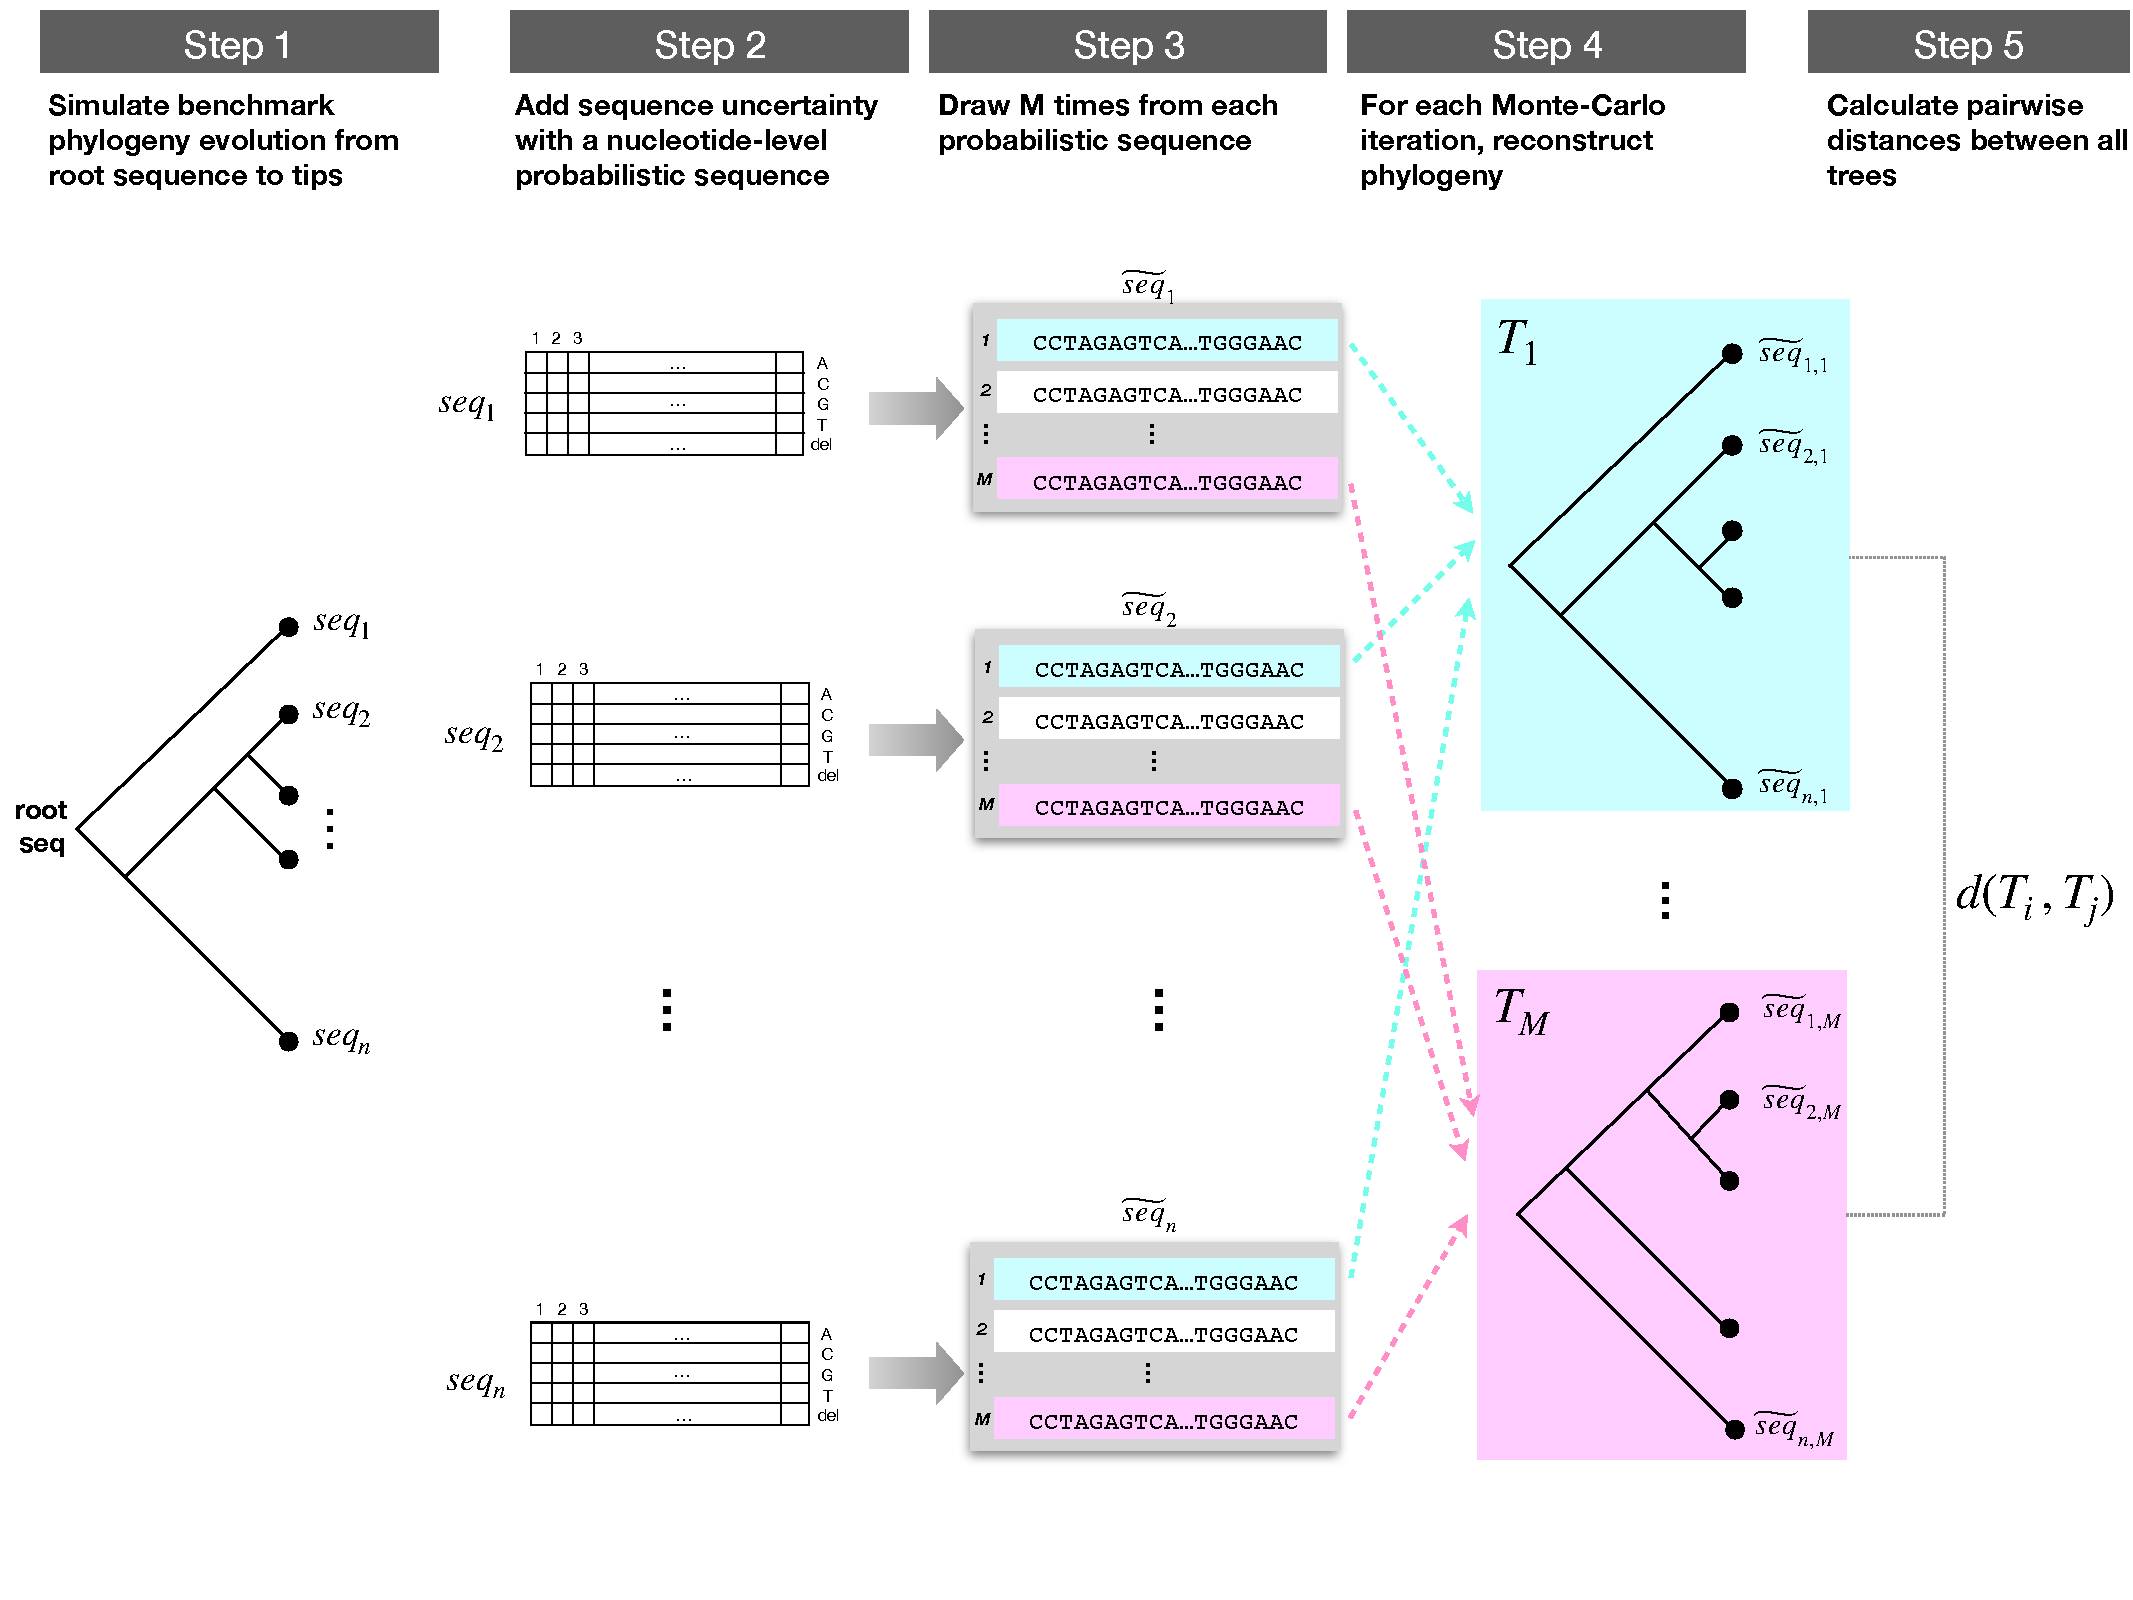
\includegraphics[width=0.99\textwidth]{figs/pipeline.pdf}
\caption{\textbf{Simulations pipeline.} 
\textit{Step 1}: A phylogeny with $n$ final nodes is simulated from a root sequence using \textsf{phylosim}.
\textit{Step 2}: A \nlps is generated for each sequence, assuming a Beta distribution for the base-call probability
\textit{Step 3}: For each \nlps, a sequence is drawn $M$ times
\textit{Step 4}: Using the ith drawn sequence (\ie ith Monte Carlo iteration), the phylogeny $T_i$ is inferred ($i=1,\ldots,M$). 
\textit{Step 5}: The pairwise distances $d(T_i, t_j)$ are calculated for all $i<j$.
Steps 1 to 5 are repeated for several level of uncertainty (defined by the Beta parameters of the base-call probabilities).
}
\label{fig:pipeline}
\end{figure}


\textbf{Impact on clustering.}
\warning{TODO}

\textbf{Impact on source attribution.}
\warning{TODO}

%Labeled distance: Tree distances are relatively ``generic''. 
%Given our phylogenic framework, more ``practical'' measure could be useful (?). 
%For example, for a given terminal node (tip, leaf) A, how does the probability that it shares a direct common ancestor with B evolve as we increase uncertainty?






\section{Results}

\newpage
\bibliography{papers}
\end{document}  